\begin{figure}
  \centering
  \begin{subfigure}[b]{0.33\textwidth}
    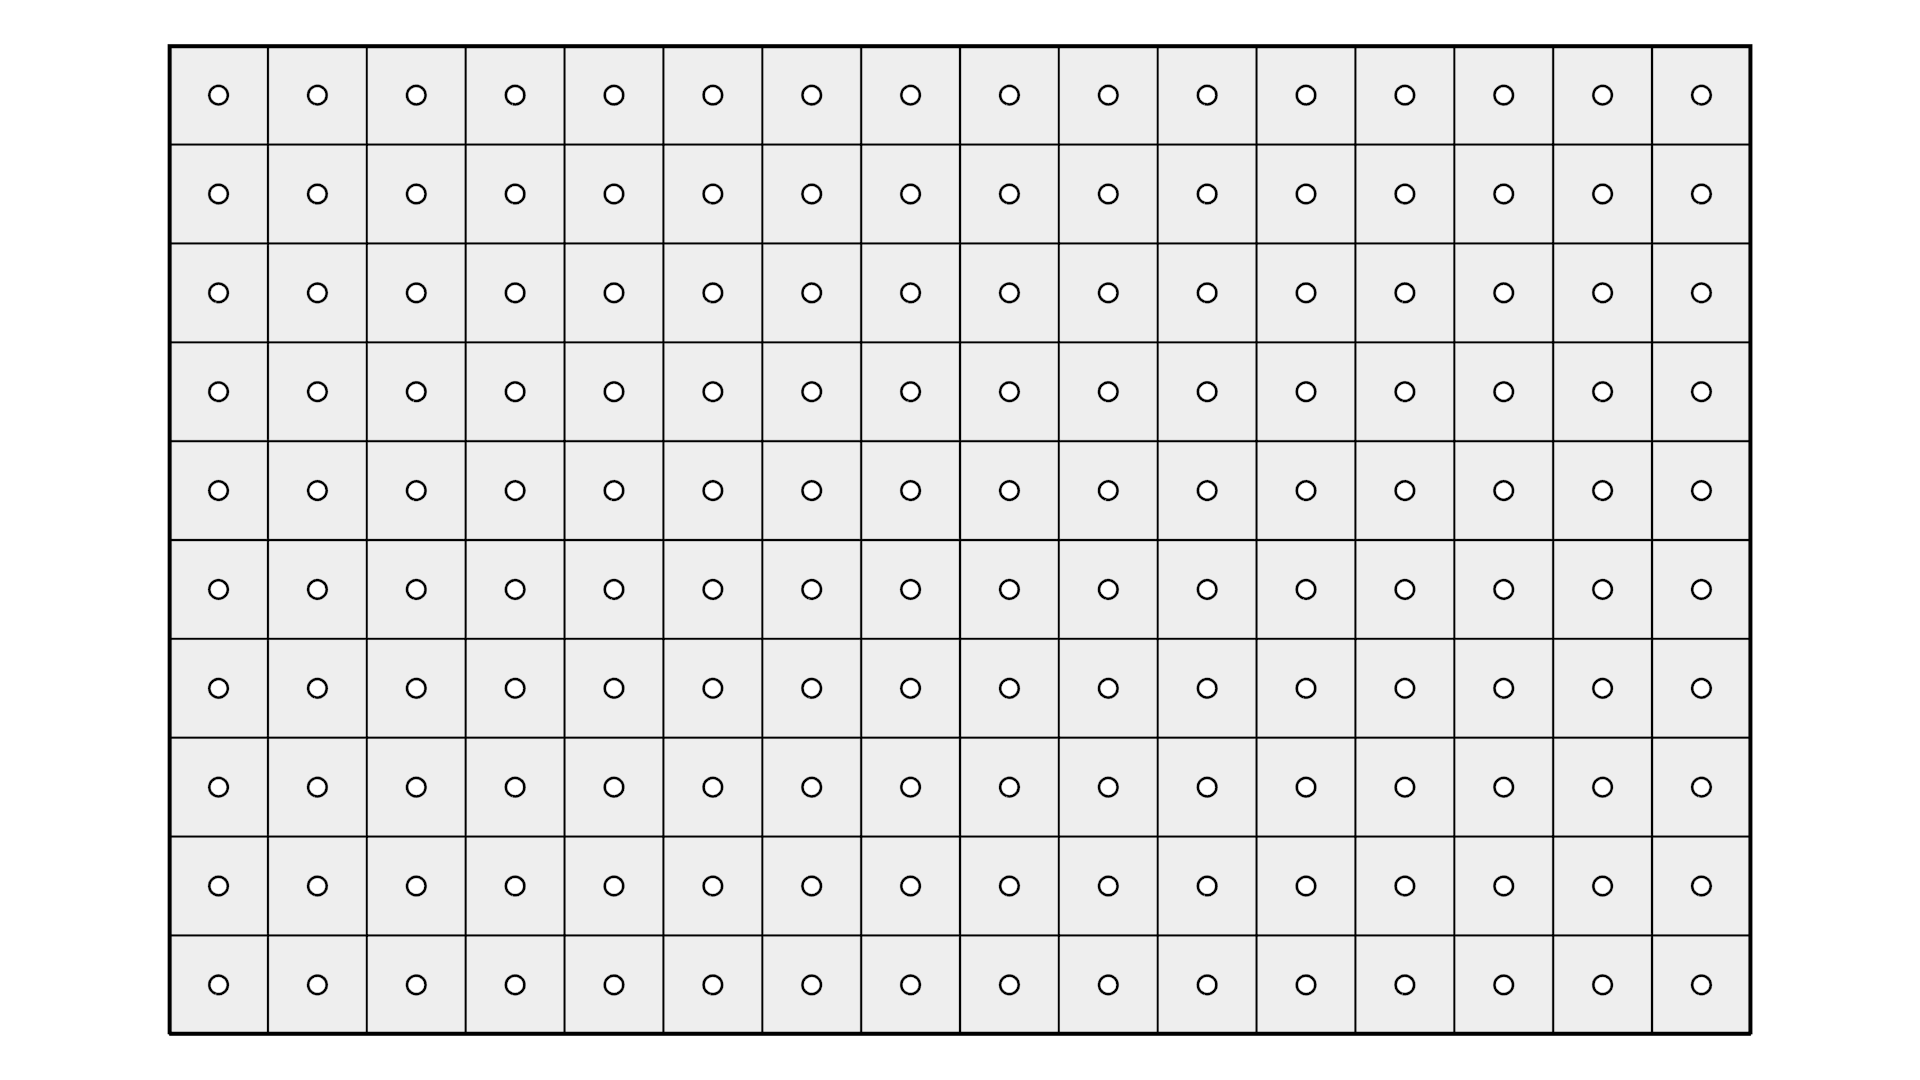
\includegraphics[width=\textwidth]{./img/raw/rt-raytracing/raytrace1.png}
    \caption{Pixeldefinitie.}
    \label{fig:rt-raytracing:1}
  \end{subfigure}%
  \begin{subfigure}[b]{0.33\textwidth}
    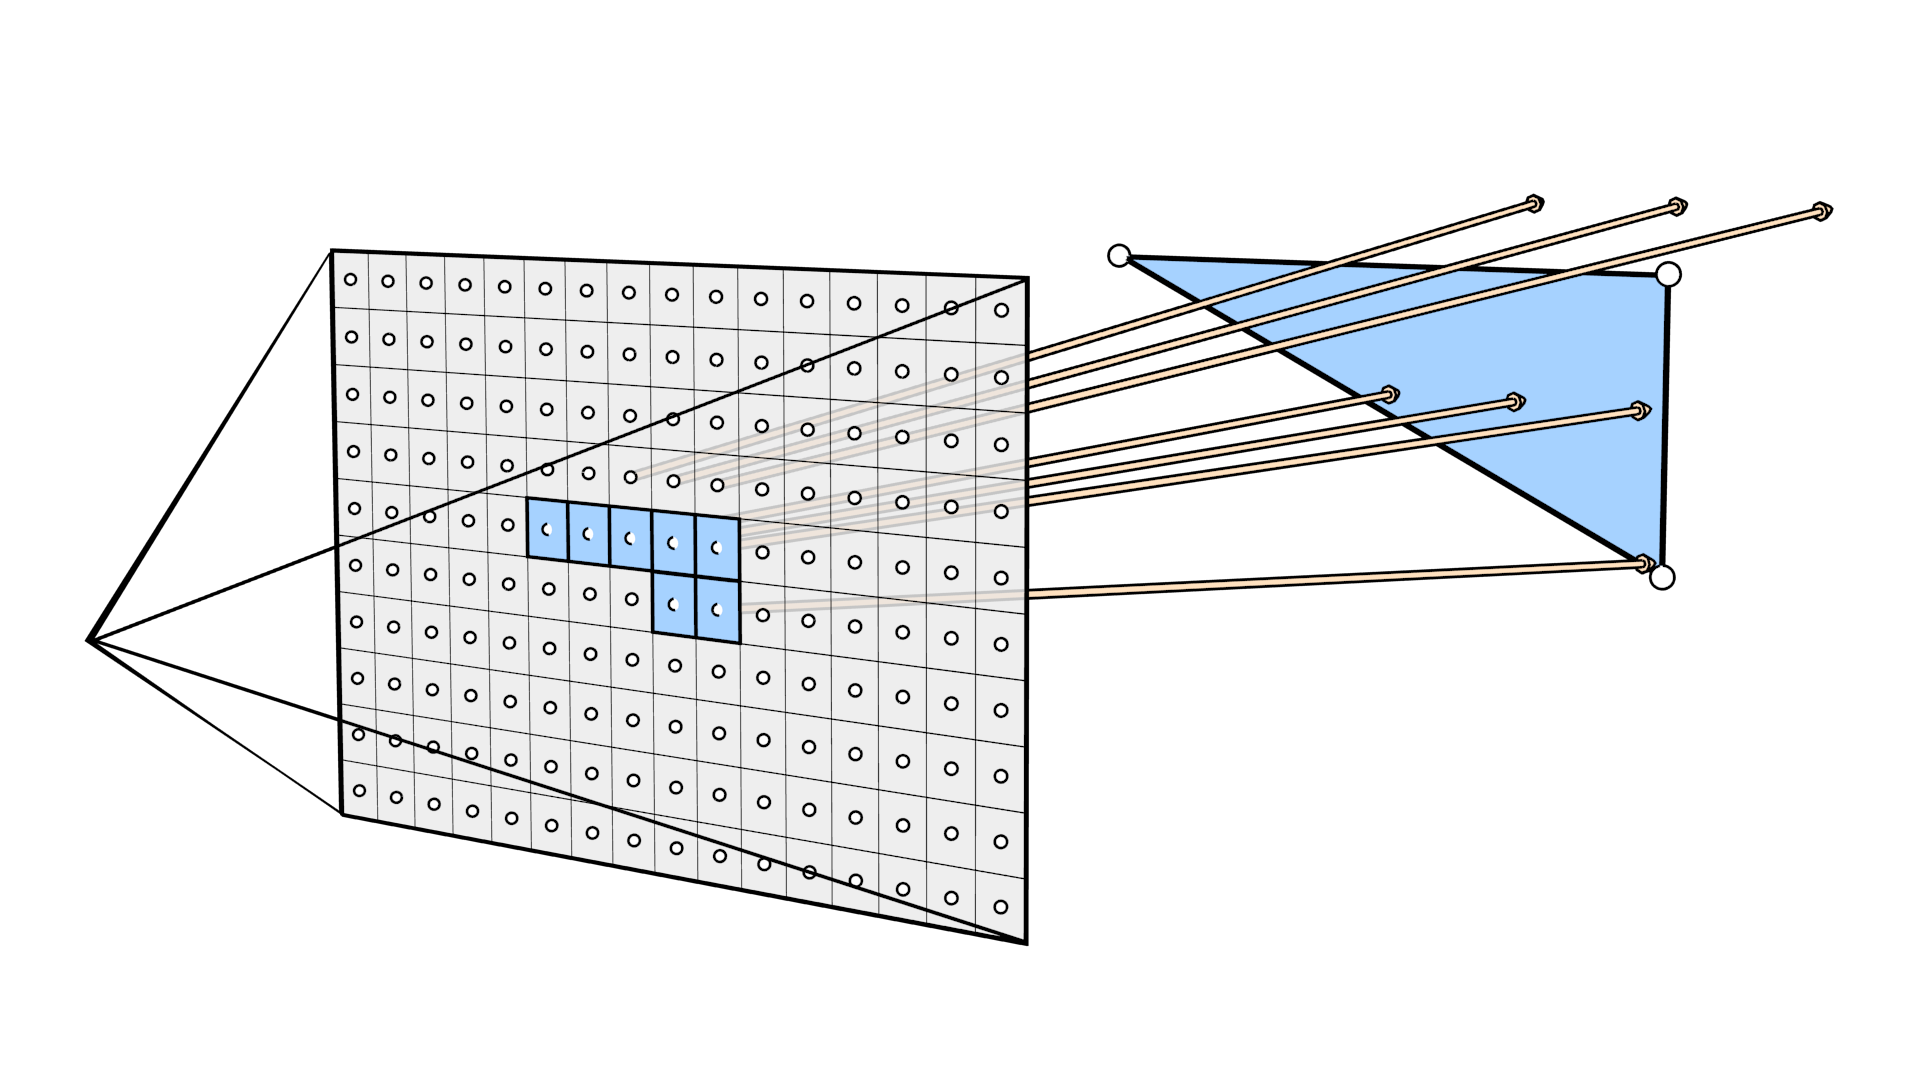
\includegraphics[width=\textwidth]{./img/raw/rt-raytracing/raytrace2.png}
    \caption{Raytracen.}
    \label{fig:rt-raytracing:2}
  \end{subfigure}%
  \begin{subfigure}[b]{0.33\textwidth}
    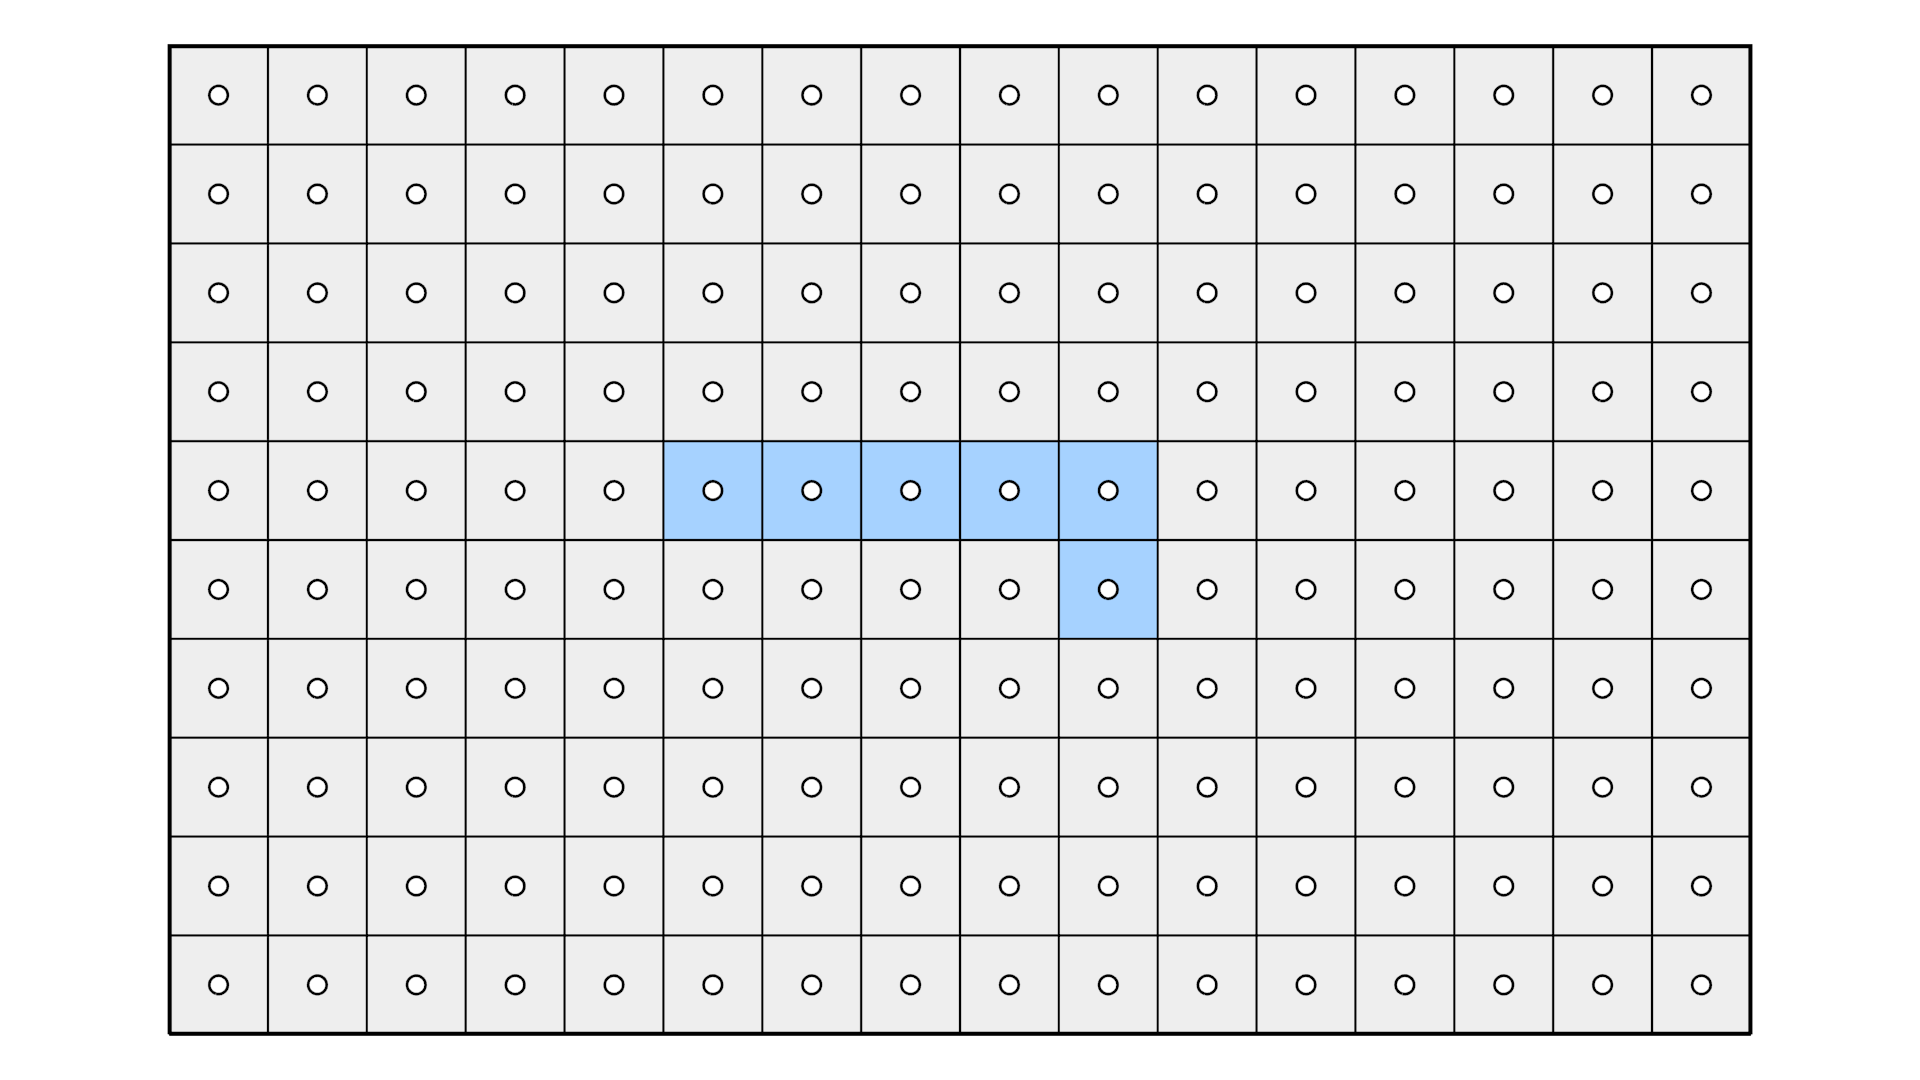
\includegraphics[width=\textwidth]{./img/raw/rt-raytracing/raytrace3.png}
    \caption{Pixeltoekenning}
    \label{fig:rt-raytracing:3}
  \end{subfigure}%
  \caption{Raytrace-algoritme.}
  \label{fig:rt-raytracing}
\end{figure}
